\chapter{Prozessmodelle}\label{sec:chapter2}

In Kapitel 2 werden grundlegende Konzepte des Software Engineering vorgestellt, die notwendig sind, um den Inhalt dieser Arbeit zu verstehen. Zunächst wird in Kapitel 2.1 der Begriff Software Engineering definiert. Weiterhin wird in Kapitel 2.2 der Begriff Softwareentwicklungsprozess erklärt. Hierbei werden Softwareprojekttypen sowie schwergewichtige und leichtgewichtige Prozessmodelle beschrieben. Anschließend gibt es eine Einführung in die drei repräsentativen Softwareentwicklungsprozesse Scrum, Open Unified Process und V-Modell-XT.

\section{Software Engineering}\label{sec:chapter2: Software Engineering}
Heutzutage werden immer mehr Systeme von Software kontrolliert \cite{Puntambekar2007}. Unter Software versteht man laut Duden die "Gesamtheit aller Programme, die auf einem Computer eingesetzt werden können". Das Wort Engineering, welches sich laut Duden von dem lateinischen Wort Ingenium [=(schöpferische) Begabung; Erfindungsgabe] ableitet, wird heutzutage mit Ingenieurwesen, bzw. technische Entwicklung übersetzt. Software Engineering umfasst somit die Gesamtheit der Aktivitäten zur Analyse, Konzeption, Entwicklung und Implementierung einer softwaretechnischen Lösung \cite{Specker1998}.
Software Engineering besteht aus mehreren Schichten (Abbildung \ref{fig:SchichtenSE}):

\begin{figure}[htp]
\begin{center}
  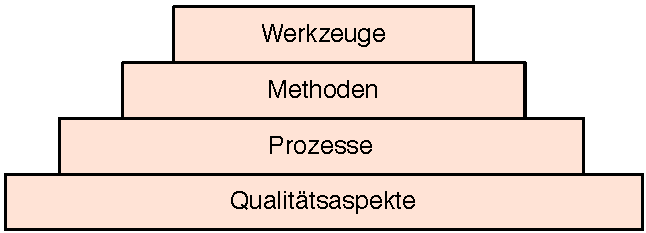
\includegraphics[width=.5\linewidth]{SELayer} %pdf, jpg, png...
  \caption{Schichten des Software Engineering \cite{Puntambekar2007}}
  \label{fig:SchichtenSE}
\end{center}
\end{figure}

Somit ist für Software Engineering in erster Linie in der Schicht Qualitätsaspekte ein diszipliniertes Qualitätsmanagement notwendig. Weiterhin ist eine Prozessschicht vorhanden, um die termingerechte Ablieferung von Software zu gewährleisten. In der Methoden-Schicht wird sodann die Implementierung unter Zuhilfenahme von Anforderungsanalysen, Design und Programmierung durchgeführt. Hierbei werden Werkzeuge zur Automatisierung in Software-Dokumentenprozessen benutzt. Software Engineering stellt somit letztendlich eine Kombination aus Prozessen, Methoden und Tools dar, um eine qualitativ hochwertige Software zu entwickeln \cite{Puntambekar2007}.

\section{Softwareentwicklungsprozesse}\label{sec:chapter.2: Softwareentwicklungsprozesse}

Für das Verständnis, die Schaffung oder Unternehmung von etwas Großem, fertigen Menschen in der Regel ein vereinfachtes Bild davon an. Hierfür nehmen sie Maß, fertigen eine Skizze oder einen Plan an oder orientieren sich an einem Vorbild, bzw. bauen sich eines. Dies geschieht normalerweise mit Papier und Schreibzeug, anderen Materialien oder einem Computer. Besonders für die Lösung von komplexen wissenschaftlichen Problemen oder bei großen Konstruktionsaufgaben ist dies unumgänglich \cite{Hesse2008}. \newline
Hierbei stützten sich die Menschen auf Modelle, welche als Stellvertreter für die Sache, die verstanden, geschaffen, unternommen oder betrieben werden soll, angesehen werden kann \cite{Hesse2008}. \newline
Insbesondere die heutzutage von Softwareentwicklern zu erstellenden Softwareprodukte zeichnen sich durch ein hohes Maß an Komplexität und Umfang aus. Neben den Erwartungen von Kunden hinsichtlich Qualität müssen Softwaresysteme ebenfalls termingerecht und innerhalb eines vorgegebenen Budgetrahmens erstellt werden. Effektive und effiziente Softwareentwicklungsprozesse gewinnen somit immer mehr an Bedeutung \cite{Grechenig2010}.
Modell leitet sich von dem lateinischen Begriff  \glqq modelus\grqq \ 
ab und kann mit  \grqq Regel, Form, Muster, Vorbild\grqq \ übersetzt werden \cite{Hesse2008}. 
Der Begriff Prozess stammt von dem lateinischen Wort "processus" ' ab und lässt sich mit "Fortgang oder Verlauf"' übersetzen \cite{koch2011, Staud2006}. \newline 
Ein Softwareprozess ist eine Abfolge von Schritten, welche zur Herstellung von Software notwendig sind \cite{Mishra2012, Stoerrle2005}. Mit Hilfe eines Softwareentwicklungsprozesses lässt sich der organisatorische Rahmen zur Herstellung von Software beschreiben \cite{Koelmel2000}. Ein Softwareentwicklungsprozess stellt somit ein Modell für die Entwicklung eines Softwaresystems dar \cite{Hanser2010}. Die einzelnen Abschnitte eines Softwareprozesses werden hierbei als Phasen bezeichnet \cite{Stoerrle2005}. Diese werden unterschieden in  \grqq Planung des Prozesses\grqq,  \grqq Spezifikation der Anforderungen an das Produkt\grqq ,  \grqq Design des Softwareprodukts\grqq,  \grqq Implementierung\grqq \ und  \grqq Diverse Tests des Softwareprodukts\grqq \ (siehe Abbildung \ref{fig:SEProzess}).

\begin{figure}[htp]
\begin{center} 
  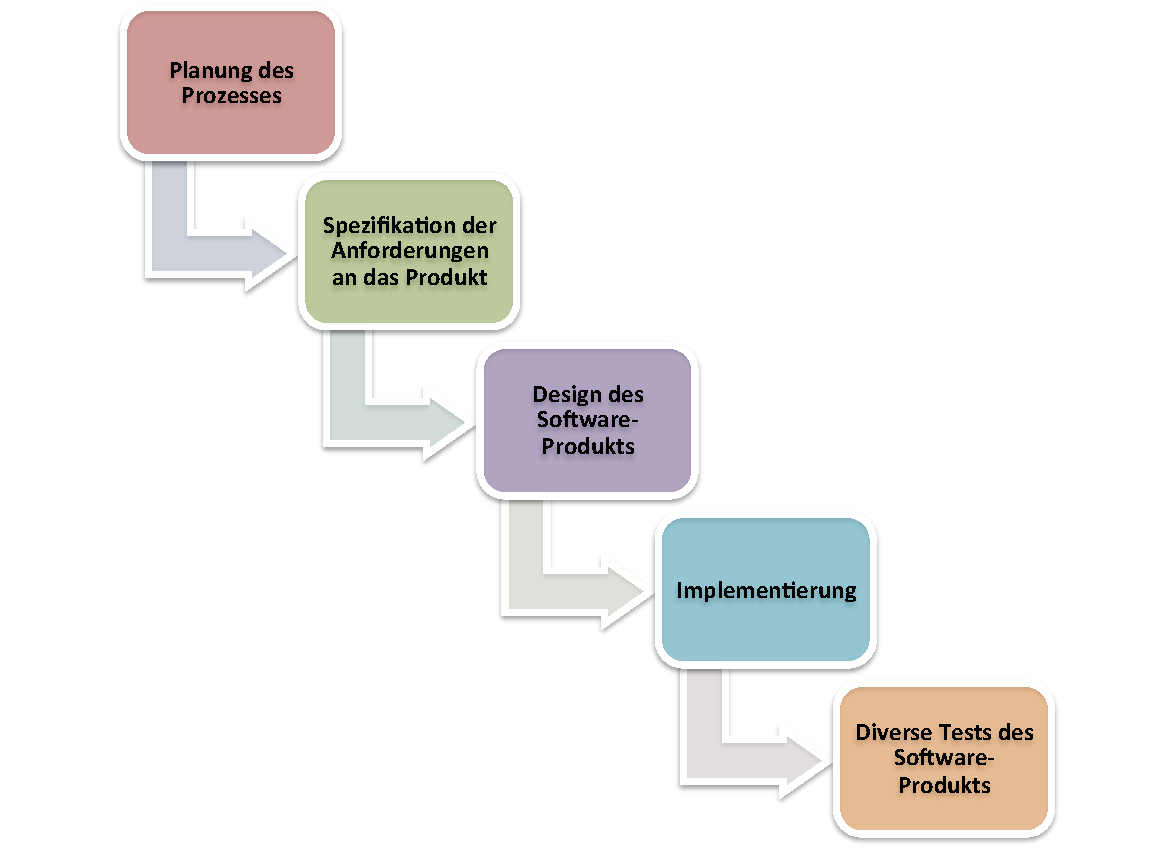
\includegraphics[width= 0.8\linewidth]{Softwareprozess} %pdf, jpg, png...
  \caption{Phasen des Softwareprozesses nach \cite{Hanser2010}}
  \label{fig:SEProzess}
\end{center}
\end{figure}

In einem Softwareentwicklungsprozess werden nicht nur die durchzuführenden Aktivitäten definiert, sondern auch die Rollen und Qualifikationen der Mitarbeiter, welche die jeweiligen Aktivitäten durchführen sollen, bzw. für diese verantwortlich sind. Des Weiteren werden die während des Entwicklungsprozesses zu erstellenden Dokumente und Unterlagen festgelegt \cite{Hanser2010}.

\subsection{Software-Projekttypen}

Software-Projekte lassen sich in drei Gruppen einteilen (siehe Abbildung \ref{fig:Projektty}):
\begin{figure}[htp]
\begin{center}
  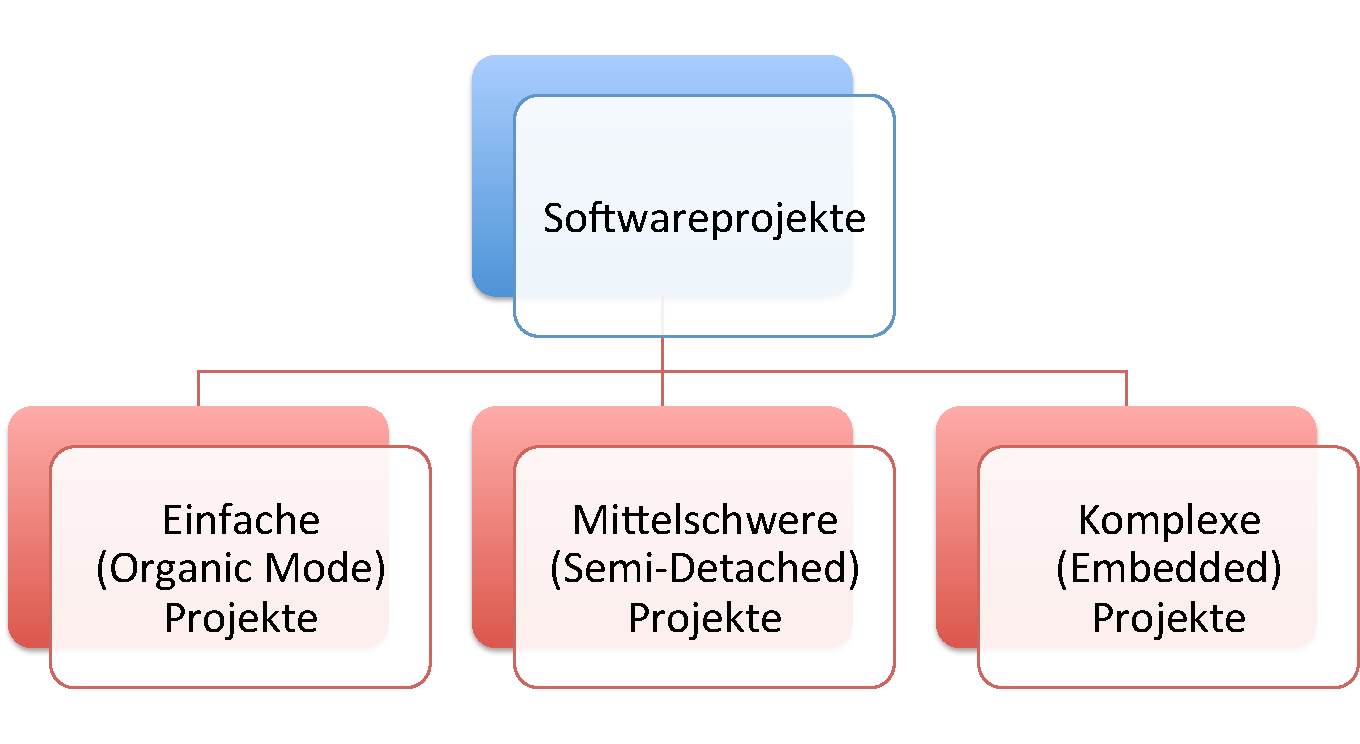
\includegraphics[width= 0.8\linewidth]{Projekttypen} %pdf, jpg, png...
  \caption{Software-Projekttypen nach \cite{Boehm81}}
  \label{fig:Projektty}
\end{center}
\end{figure}
Bei den \textit{Einfachen Projekten} sind relativ kleine Teams am Entwicklungsprozess beteiligt und bei den Teammitgliedern besteht räumliche Nähe. Jedes Teammitglied weist eine hohe methodische und fachliche Erfahrenheit auf und kennt sich in dem späteren Einsatzgebiet der Software gut aus. Die Anzahl der Code-Zeilen bei der zu entwickelnden Software ist meist gering \cite{Boehm81, Hanser2010}. \newline
Bei den \textit{Komplexen Projekten} handelt es sich um Software-Projekte, welche in den meisten Fällen stark durch behördliche Auflagen reguliert sind. Die Software muss einerseits eine hohe Zuverlässigkeit aufweisen und andererseits sind nachträgliche Änderungen fast nicht mehr möglich. Im Gegensatz zu den \textit{Einfachen Projekten} ist das Entwicklungsteam hier groß, besteht sowohl aus erfahrenen, als auch aus unerfahrenen Entwicklern und die Anzahl der Code-Zeilen ist ebenfalls groß \cite{Boehm81, Hanser2010}. \newline
Eine Schnittstelle zwischen diesen beiden Projekttypen bilden die \textit{Mittelschweren Projekte}. Hier sind die Software-Entwicklungsteams mittelgroß und bestehen aus erfahrenen und unerfahrenen Mitgliedern. Teilweise sind nicht alle Aspekte des Produktes schon im Vornherein bekannt und die Anzahl der Code-Zeilen ist groß \cite{Boehm81, Hanser2010}.

\subsection{Schwergewichtige und Leichtgewichtige Prozessmodelle}

Aus der eben erfolgten Einteilung von Software-Projekten lässt sich eine Einteilung von Software-Prozessmodellen in \textit{Leichtgewichtige} und \textit{Schwergewichtige Prozessmodelle} ableiten \cite{Hanser2010}. \newline
\textit{Leichtgewichtige Prozessmodelle} eignen sich eher für kleine Teams, bei denen keine detaillierte Anforderungserhebung stattfindet, da die Kommunikation sowohl innerhalb des Teams als auch mit dem Kunden auf Grund der kleinen Teamgröße gut funktioniert. Da viele Informationen hier informell über kurze Kommunikationswege weitergegeben werden, ist eine ausführliche Dokumentation derer nicht notwendig. \cite{Hanser2010}. \newline
Eine sehr formale und dokumentenlastige Vorgehensweise kommt bei den \textit{Schwergewichtigen Prozessmodellen} zum Einsatz. Es findet eine ausführliche Dokumentation in allen Entwicklungsphasen statt und der Ablauf des Prozesses ist genau vorgegeben. Bei Software-Produkten, welche bei einer möglichen Fehlfunktion Menschenleben in Gefahr bringen, ist beispielsweise eine Vorgehensweise mit einem \textit{Schwergewichtigen Prozessmodell} sinnvoll \cite{Hanser2010}. \newline














